% Created by tikzDevice version 0.12.6 on 2025-04-07 20:34:19
% !TEX encoding = UTF-8 Unicode
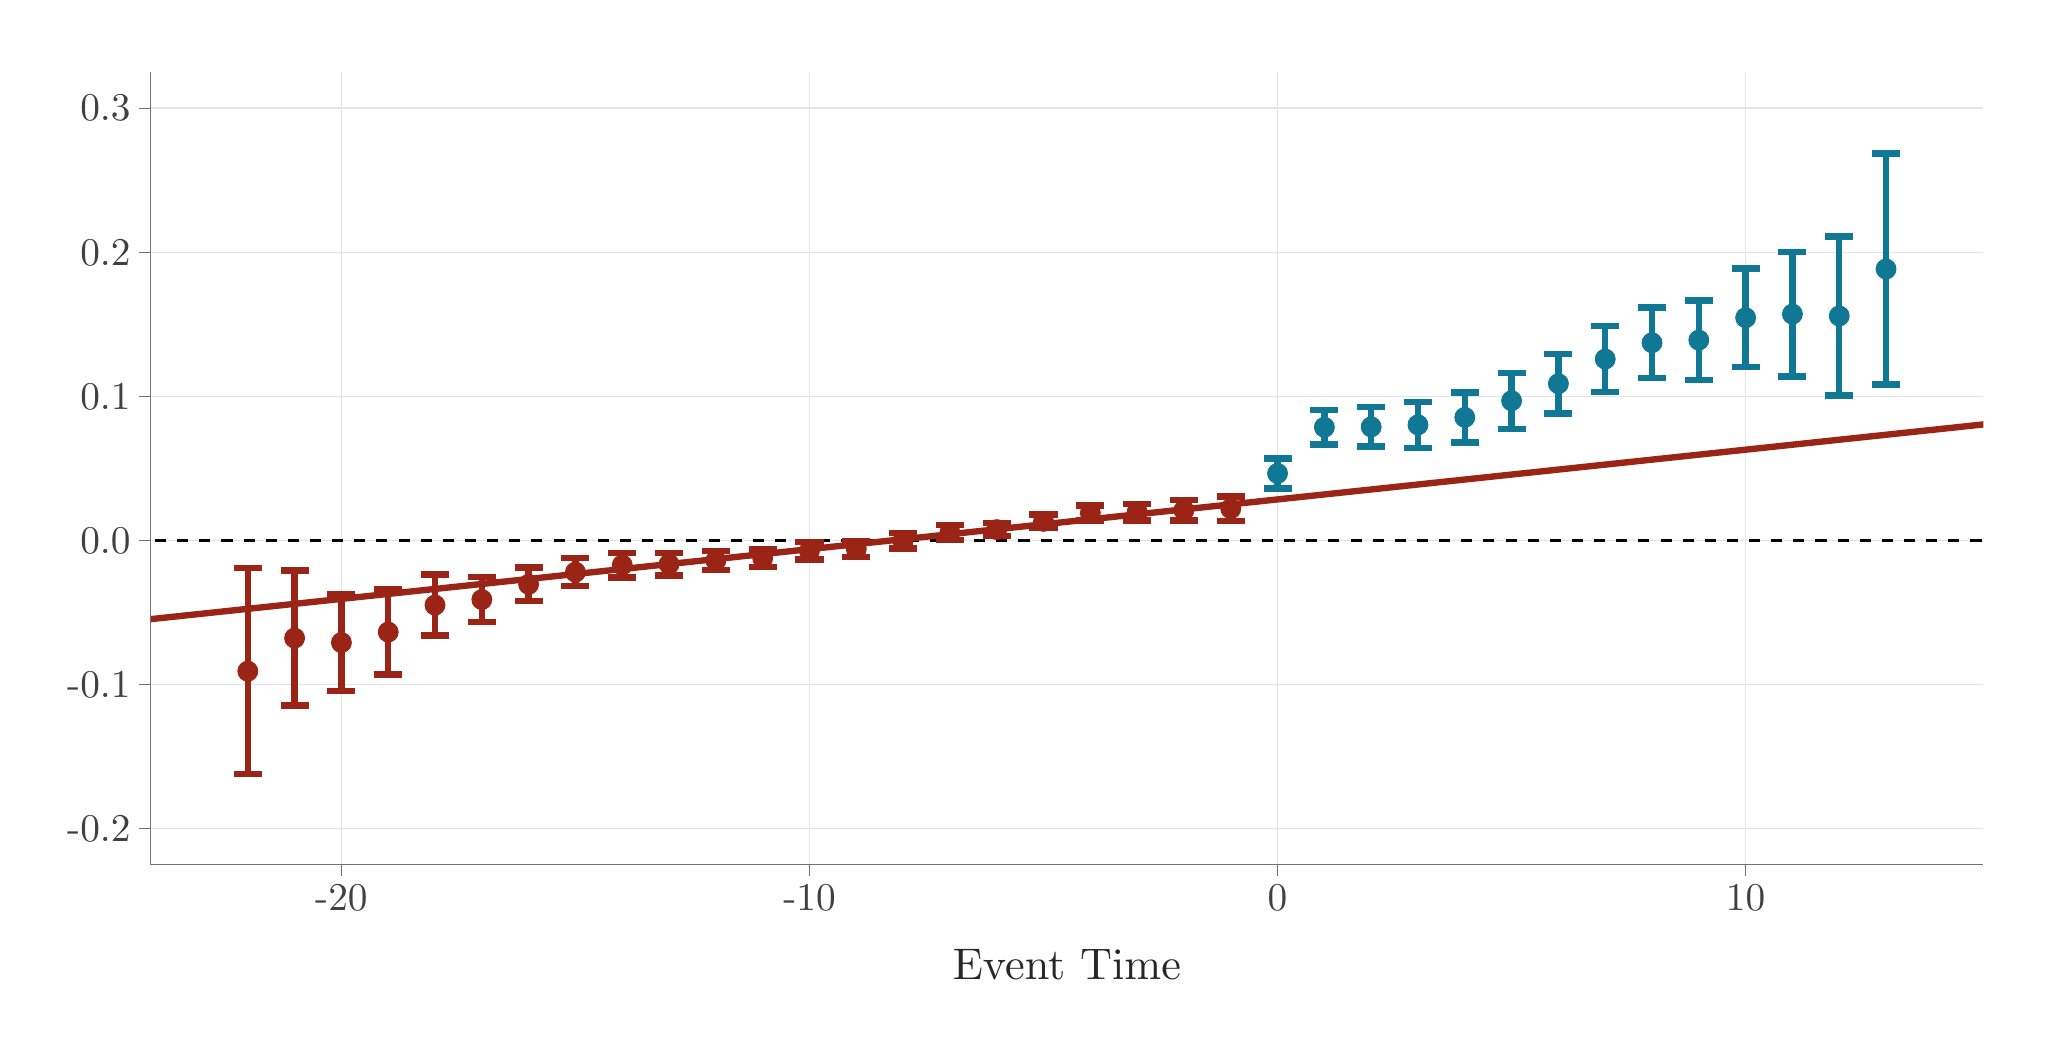
\begin{tikzpicture}[x=1pt,y=1pt]
\definecolor{fillColor}{RGB}{255,255,255}
\path[use as bounding box,fill=fillColor] (0,0) rectangle (722.70,361.35);
\begin{scope}
\path[clip] (  0.00,  0.00) rectangle (722.70,361.35);
\definecolor{drawColor}{RGB}{255,255,255}

\path[draw=drawColor,line width= 0.8pt,line join=round,line cap=round,fill=fillColor] (  0.00,  0.00) rectangle (722.70,361.35);
\end{scope}
\begin{scope}
\path[clip] ( 44.36, 58.90) rectangle (706.70,345.35);
\definecolor{drawColor}{RGB}{255,255,255}
\definecolor{fillColor}{RGB}{255,255,255}

\path[draw=drawColor,line width= 0.8pt,line join=round,line cap=round,fill=fillColor] ( 44.36, 58.90) rectangle (706.70,345.35);
\definecolor{drawColor}{RGB}{228,228,231}

\path[draw=drawColor,line width= 0.4pt,line join=round] ( 44.36, 71.92) --
	(706.70, 71.92);

\path[draw=drawColor,line width= 0.4pt,line join=round] ( 44.36,124.00) --
	(706.70,124.00);

\path[draw=drawColor,line width= 0.4pt,line join=round] ( 44.36,176.08) --
	(706.70,176.08);

\path[draw=drawColor,line width= 0.4pt,line join=round] ( 44.36,228.17) --
	(706.70,228.17);

\path[draw=drawColor,line width= 0.4pt,line join=round] ( 44.36,280.25) --
	(706.70,280.25);

\path[draw=drawColor,line width= 0.4pt,line join=round] ( 44.36,332.33) --
	(706.70,332.33);

\path[draw=drawColor,line width= 0.4pt,line join=round] (113.37, 58.90) --
	(113.37,345.35);

\path[draw=drawColor,line width= 0.4pt,line join=round] (282.50, 58.90) --
	(282.50,345.35);

\path[draw=drawColor,line width= 0.4pt,line join=round] (451.64, 58.90) --
	(451.64,345.35);

\path[draw=drawColor,line width= 0.4pt,line join=round] (620.78, 58.90) --
	(620.78,345.35);
\definecolor{drawColor}{RGB}{0,0,0}

\path[draw=drawColor,line width= 0.9pt,dash pattern=on 4pt off 4pt ,line join=round] (-617.98,176.08) -- (1369.04,176.08);
\definecolor{drawColor}{RGB}{154,36,21}

\path[draw=drawColor,line width= 2.3pt,line join=round] (-617.98, 77.23) -- (1369.04,288.36);
\definecolor{fillColor}{RGB}{154,36,21}

\path[draw=drawColor,line width= 0.4pt,line join=round,line cap=round,fill=fillColor] ( 79.54,128.82) circle (  3.57);

\path[draw=drawColor,line width= 0.4pt,line join=round,line cap=round,fill=fillColor] ( 96.45,140.78) circle (  3.57);

\path[draw=drawColor,line width= 0.4pt,line join=round,line cap=round,fill=fillColor] (113.37,139.15) circle (  3.57);

\path[draw=drawColor,line width= 0.4pt,line join=round,line cap=round,fill=fillColor] (130.28,142.95) circle (  3.57);

\path[draw=drawColor,line width= 0.4pt,line join=round,line cap=round,fill=fillColor] (147.19,152.70) circle (  3.57);

\path[draw=drawColor,line width= 0.4pt,line join=round,line cap=round,fill=fillColor] (164.11,154.69) circle (  3.57);

\path[draw=drawColor,line width= 0.4pt,line join=round,line cap=round,fill=fillColor] (181.02,160.22) circle (  3.57);

\path[draw=drawColor,line width= 0.4pt,line join=round,line cap=round,fill=fillColor] (197.94,164.61) circle (  3.57);

\path[draw=drawColor,line width= 0.4pt,line join=round,line cap=round,fill=fillColor] (214.85,167.16) circle (  3.57);

\path[draw=drawColor,line width= 0.4pt,line join=round,line cap=round,fill=fillColor] (231.76,167.50) circle (  3.57);

\path[draw=drawColor,line width= 0.4pt,line join=round,line cap=round,fill=fillColor] (248.68,168.80) circle (  3.57);

\path[draw=drawColor,line width= 0.4pt,line join=round,line cap=round,fill=fillColor] (265.59,169.66) circle (  3.57);

\path[draw=drawColor,line width= 0.4pt,line join=round,line cap=round,fill=fillColor] (282.50,172.33) circle (  3.57);

\path[draw=drawColor,line width= 0.4pt,line join=round,line cap=round,fill=fillColor] (299.42,173.00) circle (  3.57);

\path[draw=drawColor,line width= 0.4pt,line join=round,line cap=round,fill=fillColor] (316.33,175.90) circle (  3.57);

\path[draw=drawColor,line width= 0.4pt,line join=round,line cap=round,fill=fillColor] (333.25,178.90) circle (  3.57);

\path[draw=drawColor,line width= 0.4pt,line join=round,line cap=round,fill=fillColor] (350.16,179.97) circle (  3.57);

\path[draw=drawColor,line width= 0.4pt,line join=round,line cap=round,fill=fillColor] (367.07,182.95) circle (  3.57);

\path[draw=drawColor,line width= 0.4pt,line join=round,line cap=round,fill=fillColor] (383.99,186.01) circle (  3.57);

\path[draw=drawColor,line width= 0.4pt,line join=round,line cap=round,fill=fillColor] (400.90,186.32) circle (  3.57);

\path[draw=drawColor,line width= 0.4pt,line join=round,line cap=round,fill=fillColor] (417.81,186.97) circle (  3.57);

\path[draw=drawColor,line width= 0.4pt,line join=round,line cap=round,fill=fillColor] (434.73,187.52) circle (  3.57);
\definecolor{drawColor}{RGB}{16,120,149}
\definecolor{fillColor}{RGB}{16,120,149}

\path[draw=drawColor,line width= 0.4pt,line join=round,line cap=round,fill=fillColor] (451.64,200.28) circle (  3.57);

\path[draw=drawColor,line width= 0.4pt,line join=round,line cap=round,fill=fillColor] (468.56,216.96) circle (  3.57);

\path[draw=drawColor,line width= 0.4pt,line join=round,line cap=round,fill=fillColor] (485.47,217.09) circle (  3.57);

\path[draw=drawColor,line width= 0.4pt,line join=round,line cap=round,fill=fillColor] (502.38,217.83) circle (  3.57);

\path[draw=drawColor,line width= 0.4pt,line join=round,line cap=round,fill=fillColor] (519.30,220.53) circle (  3.57);

\path[draw=drawColor,line width= 0.4pt,line join=round,line cap=round,fill=fillColor] (536.21,226.53) circle (  3.57);

\path[draw=drawColor,line width= 0.4pt,line join=round,line cap=round,fill=fillColor] (553.12,232.70) circle (  3.57);

\path[draw=drawColor,line width= 0.4pt,line join=round,line cap=round,fill=fillColor] (570.04,241.60) circle (  3.57);

\path[draw=drawColor,line width= 0.4pt,line join=round,line cap=round,fill=fillColor] (586.95,247.49) circle (  3.57);

\path[draw=drawColor,line width= 0.4pt,line join=round,line cap=round,fill=fillColor] (603.86,248.45) circle (  3.57);

\path[draw=drawColor,line width= 0.4pt,line join=round,line cap=round,fill=fillColor] (620.78,256.53) circle (  3.57);

\path[draw=drawColor,line width= 0.4pt,line join=round,line cap=round,fill=fillColor] (637.69,257.85) circle (  3.57);

\path[draw=drawColor,line width= 0.4pt,line join=round,line cap=round,fill=fillColor] (654.61,257.18) circle (  3.57);

\path[draw=drawColor,line width= 0.4pt,line join=round,line cap=round,fill=fillColor] (671.52,274.15) circle (  3.57);
\definecolor{drawColor}{RGB}{154,36,21}

\path[draw=drawColor,line width= 2.3pt,line join=round] ( 74.47,165.99) --
	( 84.61,165.99);

\path[draw=drawColor,line width= 2.3pt,line join=round] ( 79.54,165.99) --
	( 79.54, 91.64);

\path[draw=drawColor,line width= 2.3pt,line join=round] ( 74.47, 91.64) --
	( 84.61, 91.64);

\path[draw=drawColor,line width= 2.3pt,line join=round] ( 91.38,165.15) --
	(101.53,165.15);

\path[draw=drawColor,line width= 2.3pt,line join=round] ( 96.45,165.15) --
	( 96.45,116.42);

\path[draw=drawColor,line width= 2.3pt,line join=round] ( 91.38,116.42) --
	(101.53,116.42);

\path[draw=drawColor,line width= 2.3pt,line join=round] (108.29,156.69) --
	(118.44,156.69);

\path[draw=drawColor,line width= 2.3pt,line join=round] (113.37,156.69) --
	(113.37,121.62);

\path[draw=drawColor,line width= 2.3pt,line join=round] (108.29,121.62) --
	(118.44,121.62);

\path[draw=drawColor,line width= 2.3pt,line join=round] (125.21,158.32) --
	(135.36,158.32);

\path[draw=drawColor,line width= 2.3pt,line join=round] (130.28,158.32) --
	(130.28,127.58);

\path[draw=drawColor,line width= 2.3pt,line join=round] (125.21,127.58) --
	(135.36,127.58);

\path[draw=drawColor,line width= 2.3pt,line join=round] (142.12,163.75) --
	(152.27,163.75);

\path[draw=drawColor,line width= 2.3pt,line join=round] (147.19,163.75) --
	(147.19,141.66);

\path[draw=drawColor,line width= 2.3pt,line join=round] (142.12,141.66) --
	(152.27,141.66);

\path[draw=drawColor,line width= 2.3pt,line join=round] (159.03,162.83) --
	(169.18,162.83);

\path[draw=drawColor,line width= 2.3pt,line join=round] (164.11,162.83) --
	(164.11,146.56);

\path[draw=drawColor,line width= 2.3pt,line join=round] (159.03,146.56) --
	(169.18,146.56);

\path[draw=drawColor,line width= 2.3pt,line join=round] (175.95,166.30) --
	(186.10,166.30);

\path[draw=drawColor,line width= 2.3pt,line join=round] (181.02,166.30) --
	(181.02,154.14);

\path[draw=drawColor,line width= 2.3pt,line join=round] (175.95,154.14) --
	(186.10,154.14);

\path[draw=drawColor,line width= 2.3pt,line join=round] (192.86,169.70) --
	(203.01,169.70);

\path[draw=drawColor,line width= 2.3pt,line join=round] (197.94,169.70) --
	(197.94,159.52);

\path[draw=drawColor,line width= 2.3pt,line join=round] (192.86,159.52) --
	(203.01,159.52);

\path[draw=drawColor,line width= 2.3pt,line join=round] (209.78,171.58) --
	(219.92,171.58);

\path[draw=drawColor,line width= 2.3pt,line join=round] (214.85,171.58) --
	(214.85,162.73);

\path[draw=drawColor,line width= 2.3pt,line join=round] (209.78,162.73) --
	(219.92,162.73);

\path[draw=drawColor,line width= 2.3pt,line join=round] (226.69,171.61) --
	(236.84,171.61);

\path[draw=drawColor,line width= 2.3pt,line join=round] (231.76,171.61) --
	(231.76,163.38);

\path[draw=drawColor,line width= 2.3pt,line join=round] (226.69,163.38) --
	(236.84,163.38);

\path[draw=drawColor,line width= 2.3pt,line join=round] (243.60,172.25) --
	(253.75,172.25);

\path[draw=drawColor,line width= 2.3pt,line join=round] (248.68,172.25) --
	(248.68,165.35);

\path[draw=drawColor,line width= 2.3pt,line join=round] (243.60,165.35) --
	(253.75,165.35);

\path[draw=drawColor,line width= 2.3pt,line join=round] (260.52,172.80) --
	(270.66,172.80);

\path[draw=drawColor,line width= 2.3pt,line join=round] (265.59,172.80) --
	(265.59,166.53);

\path[draw=drawColor,line width= 2.3pt,line join=round] (260.52,166.53) --
	(270.66,166.53);

\path[draw=drawColor,line width= 2.3pt,line join=round] (277.43,175.47) --
	(287.58,175.47);

\path[draw=drawColor,line width= 2.3pt,line join=round] (282.50,175.47) --
	(282.50,169.19);

\path[draw=drawColor,line width= 2.3pt,line join=round] (277.43,169.19) --
	(287.58,169.19);

\path[draw=drawColor,line width= 2.3pt,line join=round] (294.34,175.97) --
	(304.49,175.97);

\path[draw=drawColor,line width= 2.3pt,line join=round] (299.42,175.97) --
	(299.42,170.02);

\path[draw=drawColor,line width= 2.3pt,line join=round] (294.34,170.02) --
	(304.49,170.02);

\path[draw=drawColor,line width= 2.3pt,line join=round] (311.26,178.64) --
	(321.41,178.64);

\path[draw=drawColor,line width= 2.3pt,line join=round] (316.33,178.64) --
	(316.33,173.17);

\path[draw=drawColor,line width= 2.3pt,line join=round] (311.26,173.17) --
	(321.41,173.17);

\path[draw=drawColor,line width= 2.3pt,line join=round] (328.17,181.55) --
	(338.32,181.55);

\path[draw=drawColor,line width= 2.3pt,line join=round] (333.25,181.55) --
	(333.25,176.24);

\path[draw=drawColor,line width= 2.3pt,line join=round] (328.17,176.24) --
	(338.32,176.24);

\path[draw=drawColor,line width= 2.3pt,line join=round] (345.08,182.36) --
	(355.23,182.36);

\path[draw=drawColor,line width= 2.3pt,line join=round] (350.16,182.36) --
	(350.16,177.58);

\path[draw=drawColor,line width= 2.3pt,line join=round] (345.08,177.58) --
	(355.23,177.58);

\path[draw=drawColor,line width= 2.3pt,line join=round] (362.00,185.38) --
	(372.15,185.38);

\path[draw=drawColor,line width= 2.3pt,line join=round] (367.07,185.38) --
	(367.07,180.52);

\path[draw=drawColor,line width= 2.3pt,line join=round] (362.00,180.52) --
	(372.15,180.52);

\path[draw=drawColor,line width= 2.3pt,line join=round] (378.91,188.71) --
	(389.06,188.71);

\path[draw=drawColor,line width= 2.3pt,line join=round] (383.99,188.71) --
	(383.99,183.31);

\path[draw=drawColor,line width= 2.3pt,line join=round] (378.91,183.31) --
	(389.06,183.31);

\path[draw=drawColor,line width= 2.3pt,line join=round] (395.83,189.34) --
	(405.97,189.34);

\path[draw=drawColor,line width= 2.3pt,line join=round] (400.90,189.34) --
	(400.90,183.30);

\path[draw=drawColor,line width= 2.3pt,line join=round] (395.83,183.30) --
	(405.97,183.30);

\path[draw=drawColor,line width= 2.3pt,line join=round] (412.74,190.62) --
	(422.89,190.62);

\path[draw=drawColor,line width= 2.3pt,line join=round] (417.81,190.62) --
	(417.81,183.31);

\path[draw=drawColor,line width= 2.3pt,line join=round] (412.74,183.31) --
	(422.89,183.31);

\path[draw=drawColor,line width= 2.3pt,line join=round] (429.65,191.97) --
	(439.80,191.97);

\path[draw=drawColor,line width= 2.3pt,line join=round] (434.73,191.97) --
	(434.73,183.06);

\path[draw=drawColor,line width= 2.3pt,line join=round] (429.65,183.06) --
	(439.80,183.06);
\definecolor{drawColor}{RGB}{16,120,149}

\path[draw=drawColor,line width= 2.3pt,line join=round] (446.57,205.69) --
	(456.72,205.69);

\path[draw=drawColor,line width= 2.3pt,line join=round] (451.64,205.69) --
	(451.64,194.88);

\path[draw=drawColor,line width= 2.3pt,line join=round] (446.57,194.88) --
	(456.72,194.88);

\path[draw=drawColor,line width= 2.3pt,line join=round] (463.48,223.19) --
	(473.63,223.19);

\path[draw=drawColor,line width= 2.3pt,line join=round] (468.56,223.19) --
	(468.56,210.73);

\path[draw=drawColor,line width= 2.3pt,line join=round] (463.48,210.73) --
	(473.63,210.73);

\path[draw=drawColor,line width= 2.3pt,line join=round] (480.39,224.21) --
	(490.54,224.21);

\path[draw=drawColor,line width= 2.3pt,line join=round] (485.47,224.21) --
	(485.47,209.98);

\path[draw=drawColor,line width= 2.3pt,line join=round] (480.39,209.98) --
	(490.54,209.98);

\path[draw=drawColor,line width= 2.3pt,line join=round] (497.31,226.10) --
	(507.46,226.10);

\path[draw=drawColor,line width= 2.3pt,line join=round] (502.38,226.10) --
	(502.38,209.57);

\path[draw=drawColor,line width= 2.3pt,line join=round] (497.31,209.57) --
	(507.46,209.57);

\path[draw=drawColor,line width= 2.3pt,line join=round] (514.22,229.55) --
	(524.37,229.55);

\path[draw=drawColor,line width= 2.3pt,line join=round] (519.30,229.55) --
	(519.30,211.50);

\path[draw=drawColor,line width= 2.3pt,line join=round] (514.22,211.50) --
	(524.37,211.50);

\path[draw=drawColor,line width= 2.3pt,line join=round] (531.14,236.67) --
	(541.28,236.67);

\path[draw=drawColor,line width= 2.3pt,line join=round] (536.21,236.67) --
	(536.21,216.40);

\path[draw=drawColor,line width= 2.3pt,line join=round] (531.14,216.40) --
	(541.28,216.40);

\path[draw=drawColor,line width= 2.3pt,line join=round] (548.05,243.44) --
	(558.20,243.44);

\path[draw=drawColor,line width= 2.3pt,line join=round] (553.12,243.44) --
	(553.12,221.97);

\path[draw=drawColor,line width= 2.3pt,line join=round] (548.05,221.97) --
	(558.20,221.97);

\path[draw=drawColor,line width= 2.3pt,line join=round] (564.96,253.46) --
	(575.11,253.46);

\path[draw=drawColor,line width= 2.3pt,line join=round] (570.04,253.46) --
	(570.04,229.74);

\path[draw=drawColor,line width= 2.3pt,line join=round] (564.96,229.74) --
	(575.11,229.74);

\path[draw=drawColor,line width= 2.3pt,line join=round] (581.88,260.20) --
	(592.03,260.20);

\path[draw=drawColor,line width= 2.3pt,line join=round] (586.95,260.20) --
	(586.95,234.78);

\path[draw=drawColor,line width= 2.3pt,line join=round] (581.88,234.78) --
	(592.03,234.78);

\path[draw=drawColor,line width= 2.3pt,line join=round] (598.79,262.80) --
	(608.94,262.80);

\path[draw=drawColor,line width= 2.3pt,line join=round] (603.86,262.80) --
	(603.86,234.10);

\path[draw=drawColor,line width= 2.3pt,line join=round] (598.79,234.10) --
	(608.94,234.10);

\path[draw=drawColor,line width= 2.3pt,line join=round] (615.70,274.27) --
	(625.85,274.27);

\path[draw=drawColor,line width= 2.3pt,line join=round] (620.78,274.27) --
	(620.78,238.79);

\path[draw=drawColor,line width= 2.3pt,line join=round] (615.70,238.79) --
	(625.85,238.79);

\path[draw=drawColor,line width= 2.3pt,line join=round] (632.62,280.36) --
	(642.77,280.36);

\path[draw=drawColor,line width= 2.3pt,line join=round] (637.69,280.36) --
	(637.69,235.34);

\path[draw=drawColor,line width= 2.3pt,line join=round] (632.62,235.34) --
	(642.77,235.34);

\path[draw=drawColor,line width= 2.3pt,line join=round] (649.53,285.94) --
	(659.68,285.94);

\path[draw=drawColor,line width= 2.3pt,line join=round] (654.61,285.94) --
	(654.61,228.42);

\path[draw=drawColor,line width= 2.3pt,line join=round] (649.53,228.42) --
	(659.68,228.42);

\path[draw=drawColor,line width= 2.3pt,line join=round] (666.45,315.84) --
	(676.59,315.84);

\path[draw=drawColor,line width= 2.3pt,line join=round] (671.52,315.84) --
	(671.52,232.45);

\path[draw=drawColor,line width= 2.3pt,line join=round] (666.45,232.45) --
	(676.59,232.45);
\end{scope}
\begin{scope}
\path[clip] (  0.00,  0.00) rectangle (722.70,361.35);
\definecolor{drawColor}{RGB}{113,113,122}

\path[draw=drawColor,line width= 0.3pt,line join=round] ( 44.36, 58.90) --
	( 44.36,345.35);
\end{scope}
\begin{scope}
\path[clip] (  0.00,  0.00) rectangle (722.70,361.35);
\definecolor{drawColor}{RGB}{63,63,70}

\node[text=drawColor,anchor=base east,inner sep=0pt, outer sep=0pt, scale=  1.42] at ( 37.16, 67.26) {-0.2};

\node[text=drawColor,anchor=base east,inner sep=0pt, outer sep=0pt, scale=  1.42] at ( 37.16,119.34) {-0.1};

\node[text=drawColor,anchor=base east,inner sep=0pt, outer sep=0pt, scale=  1.42] at ( 37.16,171.42) {0.0};

\node[text=drawColor,anchor=base east,inner sep=0pt, outer sep=0pt, scale=  1.42] at ( 37.16,223.50) {0.1};

\node[text=drawColor,anchor=base east,inner sep=0pt, outer sep=0pt, scale=  1.42] at ( 37.16,275.58) {0.2};

\node[text=drawColor,anchor=base east,inner sep=0pt, outer sep=0pt, scale=  1.42] at ( 37.16,327.67) {0.3};
\end{scope}
\begin{scope}
\path[clip] (  0.00,  0.00) rectangle (722.70,361.35);
\definecolor{drawColor}{RGB}{113,113,122}

\path[draw=drawColor,line width= 0.3pt,line join=round] ( 40.36, 71.92) --
	( 44.36, 71.92);

\path[draw=drawColor,line width= 0.3pt,line join=round] ( 40.36,124.00) --
	( 44.36,124.00);

\path[draw=drawColor,line width= 0.3pt,line join=round] ( 40.36,176.08) --
	( 44.36,176.08);

\path[draw=drawColor,line width= 0.3pt,line join=round] ( 40.36,228.17) --
	( 44.36,228.17);

\path[draw=drawColor,line width= 0.3pt,line join=round] ( 40.36,280.25) --
	( 44.36,280.25);

\path[draw=drawColor,line width= 0.3pt,line join=round] ( 40.36,332.33) --
	( 44.36,332.33);
\end{scope}
\begin{scope}
\path[clip] (  0.00,  0.00) rectangle (722.70,361.35);
\definecolor{drawColor}{RGB}{113,113,122}

\path[draw=drawColor,line width= 0.3pt,line join=round] ( 44.36, 58.90) --
	(706.70, 58.90);
\end{scope}
\begin{scope}
\path[clip] (  0.00,  0.00) rectangle (722.70,361.35);
\definecolor{drawColor}{RGB}{113,113,122}

\path[draw=drawColor,line width= 0.3pt,line join=round] (113.37, 54.90) --
	(113.37, 58.90);

\path[draw=drawColor,line width= 0.3pt,line join=round] (282.50, 54.90) --
	(282.50, 58.90);

\path[draw=drawColor,line width= 0.3pt,line join=round] (451.64, 54.90) --
	(451.64, 58.90);

\path[draw=drawColor,line width= 0.3pt,line join=round] (620.78, 54.90) --
	(620.78, 58.90);
\end{scope}
\begin{scope}
\path[clip] (  0.00,  0.00) rectangle (722.70,361.35);
\definecolor{drawColor}{RGB}{63,63,70}

\node[text=drawColor,anchor=base,inner sep=0pt, outer sep=0pt, scale=  1.42] at (113.37, 42.37) {-20};

\node[text=drawColor,anchor=base,inner sep=0pt, outer sep=0pt, scale=  1.42] at (282.50, 42.37) {-10};

\node[text=drawColor,anchor=base,inner sep=0pt, outer sep=0pt, scale=  1.42] at (451.64, 42.37) {0};

\node[text=drawColor,anchor=base,inner sep=0pt, outer sep=0pt, scale=  1.42] at (620.78, 42.37) {10};
\end{scope}
\begin{scope}
\path[clip] (  0.00,  0.00) rectangle (722.70,361.35);
\definecolor{drawColor}{RGB}{39,39,42}

\node[text=drawColor,anchor=base,inner sep=0pt, outer sep=0pt, scale=  1.60] at (375.53, 17.56) {Event Time};
\end{scope}
\end{tikzpicture}
